
\begin{figure}[t] %  [tp]
\centering
  %
\tikzset{every picture/.style={line width=0.75pt}} %set default line width to 0.75pt        

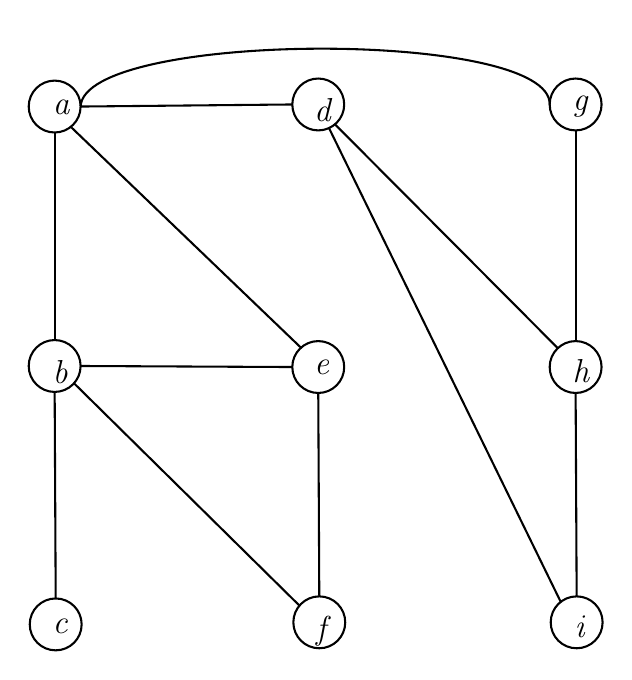
\begin{tikzpicture}%
%   [x=0.75pt,y=0.75pt,yscale=-1,xscale=1]
[x=0.75pt,y=0.75pt,yscale=-0.5,xscale=0.5]
%uncomment if require: \path (0,980); %set diagram left start at 0, and has height of 980

%Shape: Circle [id:dp4646708758113479] 
\draw   (47,126) .. controls (47,112.19) and (58.19,101) .. (72,101) .. controls (85.81,101) and (97,112.19) .. (97,126) .. controls (97,139.81) and (85.81,151) .. (72,151) .. controls (58.19,151) and (47,139.81) .. (47,126) -- cycle ;
%Shape: Circle [id:dp8478746893404502] 
\draw   (47,376) .. controls (47,362.19) and (58.19,351) .. (72,351) .. controls (85.81,351) and (97,362.19) .. (97,376) .. controls (97,389.81) and (85.81,401) .. (72,401) .. controls (58.19,401) and (47,389.81) .. (47,376) -- cycle ;
%Shape: Circle [id:dp9128600249304338] 
\draw   (48,625) .. controls (48,611.19) and (59.19,600) .. (73,600) .. controls (86.81,600) and (98,611.19) .. (98,625) .. controls (98,638.81) and (86.81,650) .. (73,650) .. controls (59.19,650) and (48,638.81) .. (48,625) -- cycle ;
%Shape: Circle [id:dp8351284500750259] 
\draw   (549,124) .. controls (549,110.19) and (560.19,99) .. (574,99) .. controls (587.81,99) and (599,110.19) .. (599,124) .. controls (599,137.81) and (587.81,149) .. (574,149) .. controls (560.19,149) and (549,137.81) .. (549,124) -- cycle ;
%Shape: Circle [id:dp5950758015237675] 
\draw   (549,377) .. controls (549,363.19) and (560.19,352) .. (574,352) .. controls (587.81,352) and (599,363.19) .. (599,377) .. controls (599,390.81) and (587.81,402) .. (574,402) .. controls (560.19,402) and (549,390.81) .. (549,377) -- cycle ;
%Shape: Circle [id:dp49528230279796914] 
\draw   (550,623) .. controls (550,609.19) and (561.19,598) .. (575,598) .. controls (588.81,598) and (600,609.19) .. (600,623) .. controls (600,636.81) and (588.81,648) .. (575,648) .. controls (561.19,648) and (550,636.81) .. (550,623) -- cycle ;
%Shape: Circle [id:dp25484460537469966] 
\draw   (301,124) .. controls (301,110.19) and (312.19,99) .. (326,99) .. controls (339.81,99) and (351,110.19) .. (351,124) .. controls (351,137.81) and (339.81,149) .. (326,149) .. controls (312.19,149) and (301,137.81) .. (301,124) -- cycle ;
%Shape: Circle [id:dp5057593817920109] 
\draw   (301,377) .. controls (301,363.19) and (312.19,352) .. (326,352) .. controls (339.81,352) and (351,363.19) .. (351,377) .. controls (351,390.81) and (339.81,402) .. (326,402) .. controls (312.19,402) and (301,390.81) .. (301,377) -- cycle ;
%Shape: Circle [id:dp7259219306283751] 
\draw   (302,623) .. controls (302,609.19) and (313.19,598) .. (327,598) .. controls (340.81,598) and (352,609.19) .. (352,623) .. controls (352,636.81) and (340.81,648) .. (327,648) .. controls (313.19,648) and (302,636.81) .. (302,623) -- cycle ;
%Straight Lines [id:da024699056897478644] 
\draw    (97,126) -- (301,124) ;
%Straight Lines [id:da7628340988725923] 
\draw    (72,151) -- (72,351) ;
%Straight Lines [id:da32471807104298844] 
\draw    (88,146) -- (310,359) ;
%Curve Lines [id:da3016950037979529] 
\draw    (97,126) .. controls (100,53) and (551,51) .. (549,124) ;
%Straight Lines [id:da751870944514893] 
\draw    (72,401) -- (73,600) ;
%Straight Lines [id:da9473518215611916] 
\draw    (91,393) -- (308,607) ;
%Straight Lines [id:da580665576346275] 
\draw    (326,402) -- (327,598) ;
%Straight Lines [id:da4050680129871884] 
\draw    (342,143) -- (557,359) ;
%Straight Lines [id:da4701786783304761] 
\draw    (574,149) -- (574,352) ;
%Straight Lines [id:da441628122369529] 
\draw    (336,146) -- (560,604) ;
%Straight Lines [id:da450581824363979] 
\draw    (97,376) -- (301,377) ;
%Straight Lines [id:da5469470951513473] 
\draw    (574,402) -- (575,598) ;

% Text Node
\draw (67,117) node [anchor=north west][inner sep=0.75pt]   [align=left] {{\textit{\large a}}};
% Text Node
\draw (67,368) node [anchor=north west][inner sep=0.75pt]   [align=left] {{\textit{\large b}}};
% Text Node
\draw (67,617) node [anchor=north west][inner sep=0.75pt]   [align=left] {{\textit{\large c}}};
% Text Node
\draw (319,115) node [anchor=north west][inner sep=0.75pt]   [align=left] {{\textit{\large d}}};
% Text Node
\draw (319,367) node [anchor=north west][inner sep=0.75pt]   [align=left] {{\textit{\large e}}};
% Text Node
\draw (321,614) node [anchor=north west][inner sep=0.75pt]   [align=left] {{\textit{\large f}}};
% Text Node
\draw (568,113) node [anchor=north west][inner sep=0.75pt]   [align=left] {{\textit{\large g}}};
% Text Node
\draw (568,367) node [anchor=north west][inner sep=0.75pt]   [align=left] {{\textit{\large h}}};
% Text Node
\draw (570,614) node [anchor=north west][inner sep=0.75pt]   [align=left] {{\textit{\large i}}};


\end{tikzpicture}
  %
  \caption{Undirected unweighted graph for graph traversals in
    Problem~\ref{problem:traversal}.
  }
  \label{fig:traversal}
\end{figure}
